\def\dlt{0.4}
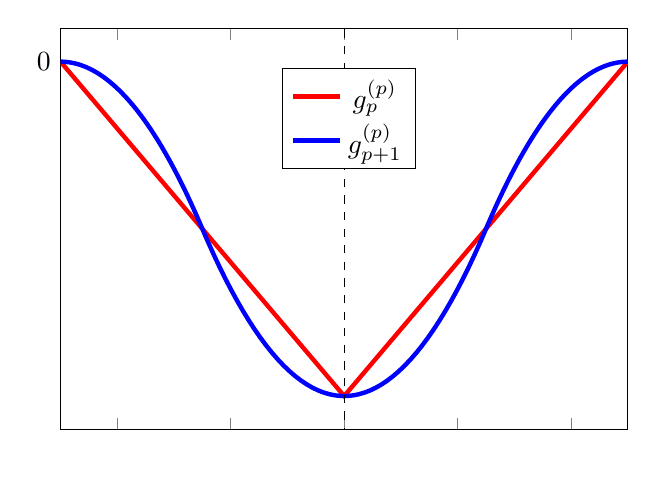
\begin{tikzpicture}
\begin{axis}[
    width=250pt,height=190pt,
    xmin=-0.5,xmax=+0.5,
    ymin=-0.55,ymax=0.05,
    samples=50,
    xtick={},
    xticklabels={},
    ytick={0},
    yticklabels={$0$},
    grid style={line width=.1pt, draw=gray!10},
    legend style={at={(0.39,0.9)}, anchor=north west}]

    \addplot[red, ultra thick] coordinates {
        (-0.5, 0) (0, -0.5) (0.5,0)
    };

    \addplot[blue, ultra thick, domain=-0.5:-0.25] (x, {-4*x*x-4*x-1});
    \legend{$g^{(p)}_p$, $g^{(p)}_{p+1}$}
    \addplot[blue, ultra thick, domain=-0.25:0.25] (x, {4*x*x-0.5});
    \addplot[blue, ultra thick, domain=0.25:0.5] (x, {-4*x*x+4*x-1});
    

    \draw [dashed] (axis cs:{0},-2) -- (axis cs:{0},2);
    
    \node at (axis cs:2.9,1.1) {$g^{(3)}_3$};
\end{axis}
\end{tikzpicture}
\undef\dlt